\documentclass[a4paper]{article}

\usepackage[utf8]{inputenc}

\usepackage{array}

% taille carte 55 mm x 80 mm

\usepackage{graphicx}
\graphicspath{ {./images/} }

\newcommand{\illusExploration}{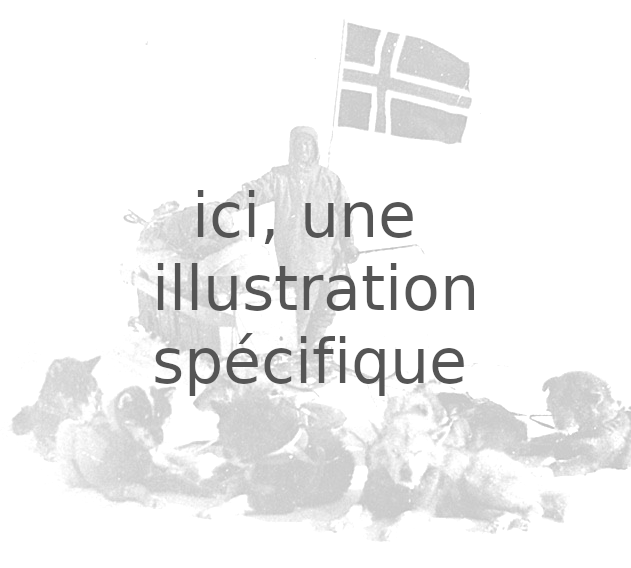
\includegraphics[width=50mm, height=3cm]{illustration_exploration}}
\newcommand{\illusPreparation}{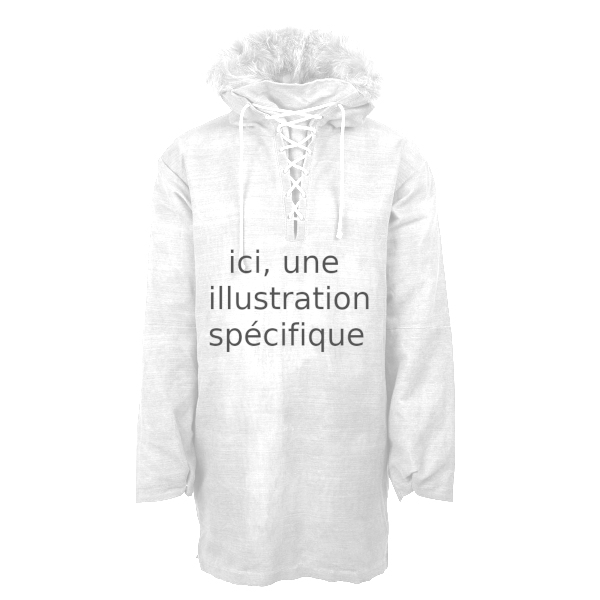
\includegraphics[width=35mm, height=3cm]{illustration_preparation}}

\newcommand{\iconeVide}{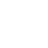
\includegraphics[width=10mm, height=10mm]{images/icones/vide_black_24dp.png}}
\newcommand{\iconeEffet}{\includegraphics[width=10mm, height=10mm]{material-design-icons/png/navigation/east/materialicons/24dp/2x/baseline_east_black_24dp.png}}
\newcommand{\iconeOu}{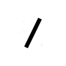
\includegraphics[width=10mm, height=10mm]{images/icones/ou_black_24dp.png}}
\newcommand{\iconeAutresJoueurs}{\includegraphics[width=10mm, height=10mm]{material-design-icons/png/social/groups/materialicons/24dp/2x/baseline_groups_black_24dp.png}}

\newcommand{\iconeSacADos}{\includegraphics[width=10mm, height=10mm]{material-design-icons/png/places/backpack/materialicons/24dp/2x/baseline_backpack_black_24dp.png}}

\newcommand{\iconeCapitaine}{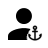
\includegraphics[width=10mm, height=10mm]{images/icones/capitaine.png}}
\newcommand{\iconeBateau}{\includegraphics[width=10mm, height=10mm]{material-design-icons//png/maps/directions_boat/materialiconsround/24dp/2x/round_directions_boat_black_24dp.png}}

\newcommand{\iconeChien}{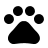
\includegraphics[width=10mm, height=10mm]{material-design-icons/png/action/pets/materialicons/24dp/2x/baseline_pets_black_24dp.png}}
\newcommand{\iconeFinChien}{
\includegraphics[width=10mm, height=10mm]{images/icones/baseline_pets_off_black_24dp.png}}

\newcommand{\iconeNourriture}{\includegraphics[width=10mm, height=10mm]{material-design-icons/png/maps/restaurant/materialicons/24dp/2x/baseline_restaurant_black_24dp.png}}
\newcommand{\iconeFinNourriture}{\includegraphics[width=10mm, height=10mm]{material-design-icons/png/maps/no_meals/materialicons/24dp/2x/baseline_no_meals_black_24dp.png}}

\newcommand{\iconeTraineau}{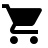
\includegraphics[width=10mm, height=10mm]{material-design-icons/png/action/shopping_cart/materialicons/24dp/2x/baseline_shopping_cart_black_24dp.png}}
\newcommand{\iconeFinTraineau}{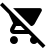
\includegraphics[width=10mm, height=10mm]{material-design-icons/png/action/remove_shopping_cart/materialicons/24dp/2x/baseline_remove_shopping_cart_black_24dp.png}}

\newcommand{\iconeHomme}{\includegraphics[width=10mm, height=10mm]{material-design-icons/png/social/person/materialicons/24dp/2x/baseline_person_black_24dp.png}}
\newcommand{\iconeFinHomme}{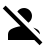
\includegraphics[width=10mm, height=10mm]{images/icones/baseline_person_off_black_24dp.png}}

\newcommand{\iconeArme}{\includegraphics[width=10mm, height=10mm]{material-design-icons/png/hardware/security/materialicons/24dp/2x/baseline_security_black_24dp.png}}

% https://icons8.com/icon/7425/beanie
% https://icons8.com/icon/6195/coat
\newcommand{\iconeVetement}{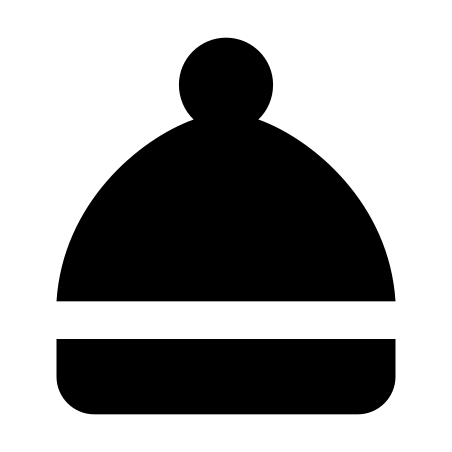
\includegraphics[width=10mm, height=10mm]{images/icones/beanie.png}}

\newcommand{\iconeExplore}{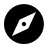
\includegraphics[width=10mm, height=10mm]{material-design-icons/png/action/explore/materialicons/24dp/2x/baseline_explore_black_24dp.png}}

\newcommand{\iconeDeplacement}{\includegraphics[width=10mm, height=10mm]{material-design-icons/png/maps/directions_walk/materialicons/24dp/2x/baseline_directions_walk_black_24dp.png}}
\newcommand{\iconeFinDeplacement}{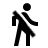
\includegraphics[width=10mm, height=10mm]{images/icones/walk_off.png}}

\newcommand{\iconeTempete}{\includegraphics[width=10mm, height=10mm]{material-design-icons/png/places/ac_unit/materialicons/24dp/2x/baseline_ac_unit_black_24dp.png}}



\pagenumbering{gobble}

\begin{document}
\begin{table}[ht]
  \begin{center}
    \caption{Préparation}
    \begin{tabular}{cccccc}
      \hline
      \textbar & \textbf{Husky} & \textbar & \textbar & \textbf{Nourriture} & \textbar\\
      \textbar &  & \textbar & \textbar &  & \textbar\\
      \textbar & \illusPreparation & \textbar & \textbar & \illusPreparation & \textbar\\
      \textbar &  & \textbar & \textbar & & \textbar\\
      \textbar &  & \textbar &\textbar & & \textbar\\
      \textbar &  & \textbar & \textbar &  & \textbar\\
      \iconeChien & \iconeVide & \iconeChien & \iconeChien & \iconeNourriture & \iconeVide\\
      \textbar &  & \textbar & \textbar &  & \textbar\\
      \hline
      \textbar & \textbf{Husky} & \textbar & \textbar & \textbf{Traineau} & \textbar\\
      \textbar &  & \textbar & \textbar &  & \textbar\\
      \textbar & \illusPreparation & \textbar & \textbar & \illusPreparation & \textbar\\
      \textbar &  & \textbar & & & \textbar\\
      \textbar &  & \textbar & \textbar & & \textbar\\
      \textbar &  & \textbar & \textbar &  & \textbar\\
      \textbar & \iconeChien & \textbar & \iconeNourriture & \iconeTraineau & \iconeNourriture\\
      \textbar &  & \textbar & \textbar &  & \textbar\\
      \hline
      \textbar & \textbf{Roald Admunsen} & \textbar & \textbar & \textbf{Gjoa} & \textbar\\
      \textbar &  & \textbar & \textbar &  & \textbar\\
      \textbar & \illusPreparation & \iconeNourriture & \iconeNourriture & \illusPreparation & \textbar\\
      \textbar &  & \textbar & \textbar & & \textbar\\
      \textbar &  & \iconeNourriture & \iconeExplore &  & \\
      \textbar &  & \textbar & \textbar &  & \textbar\\
      \textbar & \iconeCapitaine & \textbar & \textbar & \iconeBateau & \textbar\\
      \textbar &  & \textbar & \textbar &  & \textbar\\
      \hline
    \end{tabular}
  \end{center}
\end{table}

\begin{table}[ht]
  \begin{center}
    \caption{Préparation}
    \begin{tabular}{cccccc}
      \hline
      \textbar & \textbf{Équipement} & \textbar & \textbar & \textbf{Nourriture} & \textbar\\
      \iconeVide &  & \textbar & \textbar &  & \textbar\\
      \textbar & \illusPreparation & \textbar & \textbar & \illusPreparation & \textbar\\
      \textbar &  & \textbar & \textbar &  & \textbar\\
      \textbar &  & \textbar &\textbar &  & \textbar\\
      \textbar &  & \textbar & \textbar &  & \textbar\\
      \textbar & \iconeArme \iconeOu \iconeVetement & \textbar & \iconeChien & \iconeNourriture & \iconeVide\\
      \textbar &  & \textbar & \textbar &  & \textbar\\
      \hline
      \textbar & \textbf{Husky} & \textbar & \textbar & \textbf{Traineau} & \textbar\\
      \textbar &  & \textbar & \textbar &  & \textbar\\
      \textbar & \illusPreparation & \textbar & \textbar & \illusPreparation & \textbar\\
      \textbar &  & \textbar & &  & \textbar\\
      \textbar &  & \textbar & \textbar & & \textbar\\
      \textbar &  & \textbar & \textbar &  & \textbar\\
      \textbar & \iconeChien & \textbar & \iconeNourriture & \iconeTraineau & \iconeNourriture\\
      \textbar &  & \textbar & \textbar &  & \textbar\\
      \hline
      \textbar & \textbf{Robert Peary} & \textbar & \textbar & \textbf{Homme} & \textbar\\
      \textbar &  & \textbar & \textbar &  & \textbar\\
      \iconeSacADos & \illusPreparation & \iconeNourriture & \textbar & \illusPreparation & \textbar\\
      \textbar &  & \textbar & \textbar &  & \textbar\\
      \textbar &  & \iconeNourriture & \textbar &  & \\
      \textbar &  & \textbar & \textbar &  & \textbar\\
      \textbar & \iconeCapitaine & \textbar & \textbar & \iconeHomme & \textbar\\
      \textbar &  & \textbar & \textbar &  & \textbar\\
      \hline
    \end{tabular}
  \end{center}
\end{table}

\end{document}
